\chapter{Analyse de données }

\section{Nombre de nœuds}
\subsection{Par tour}
\flushleft Pour pouvoir analyser le nombre de nœuds explorés pendant une partie par un joueur utilisant MinMax,
nous avons implémenter une interface graphique qui trace une courbe à la fin de la partie.
Nous avons donc lancé plusieurs parties puis nous avons tracé les courbes suivant le nombre de tour.
Les courbes suivantes sont des courbes représentant le nombre total de nœuds parcourus par tour ainsi 
que les courbes représentant le nombre de nœuds à chaque tours.

On voit sur les premières types de courbes que au début de la partie il n'y a pas beaucoup de nœuds
parcourus car il y a peu de pions sur la grille donc peu de possibilités. Ensuite le nombre de nœuds
accélère rapidement car il y a de plus en plus de possibilités. A la fin de la partie le nombre de nœuds
redescend car il n'y a plus beaucoup de place libres dans la grille donc peu de coups valides.


\begin{figure}[!ht]
\begin{center}
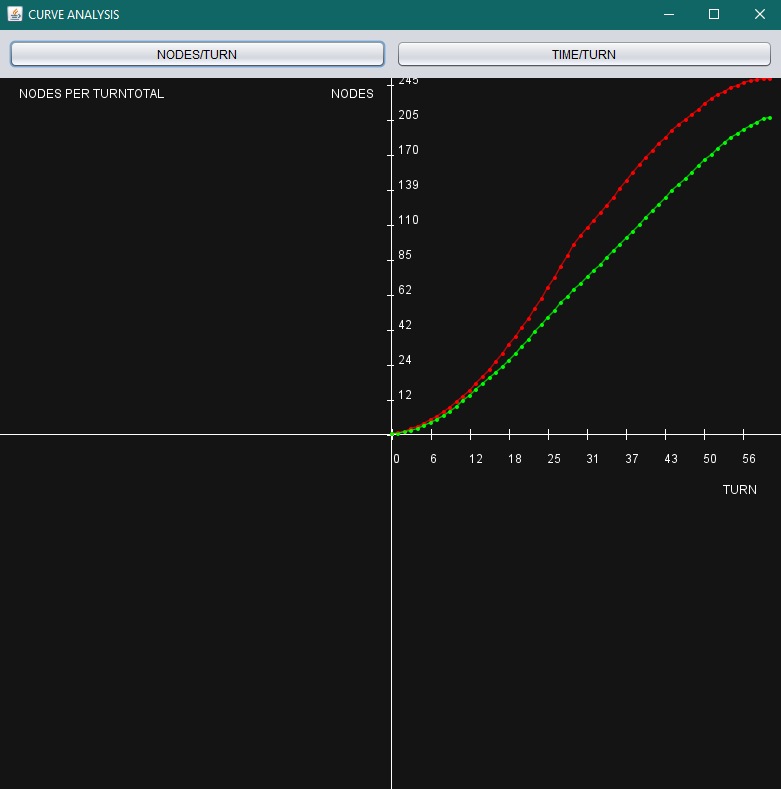
\includegraphics[width=0.60\textwidth]{./NODESPERTURN0}
\end{center}
\end{figure}
\newpage

\begin{figure}[!ht]
\begin{center}
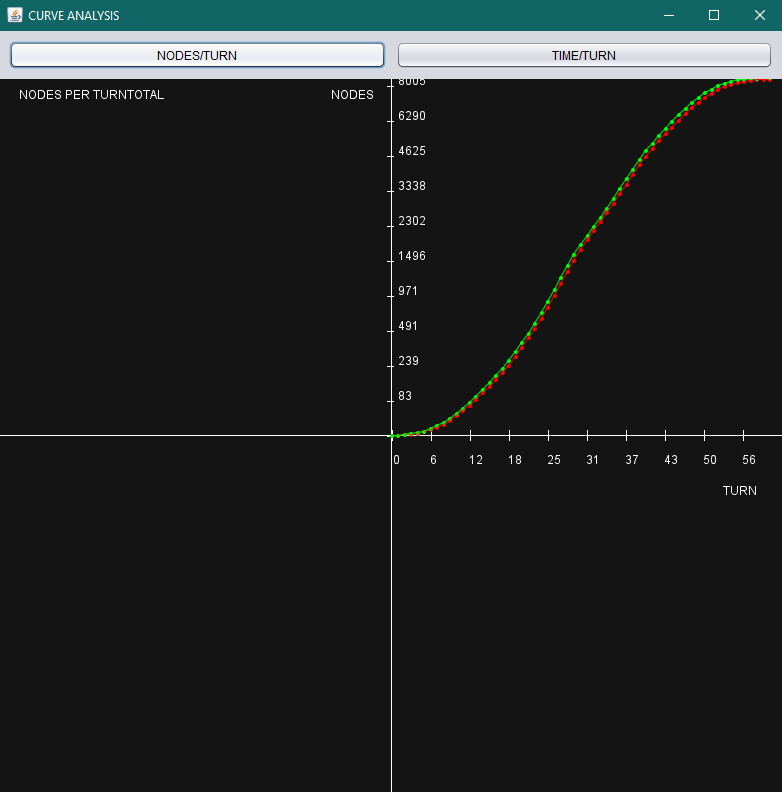
\includegraphics[width=0.60\textwidth]{./NODESPERTURN1}
\end{center}
\end{figure}

\begin{figure}[!ht]
\begin{center}
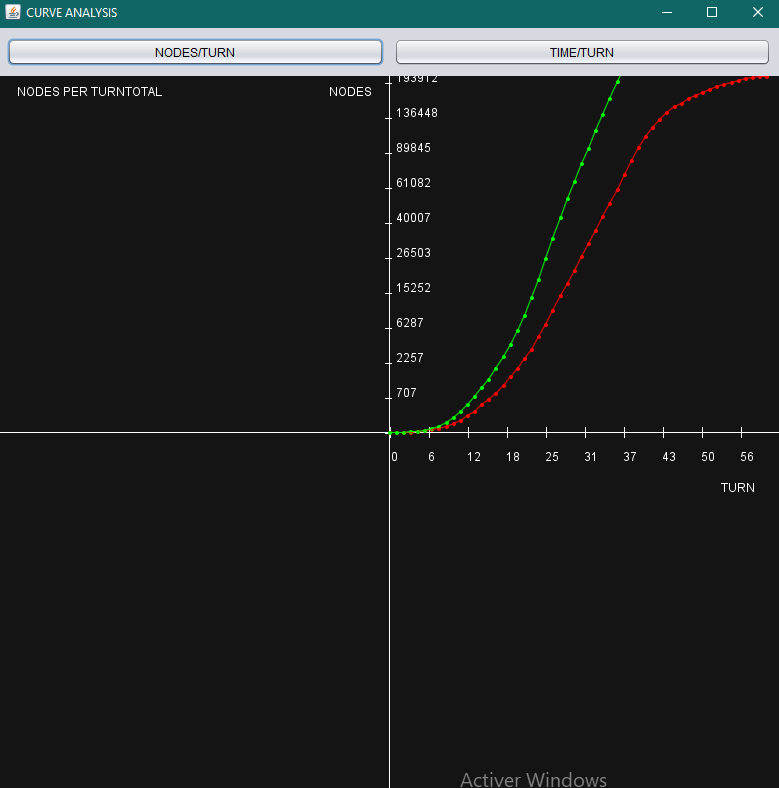
\includegraphics[width=0.60\textwidth]{./NODESPERTURN2}
\end{center}
\end{figure}
\newpage

\begin{figure}[!ht]
\begin{center}
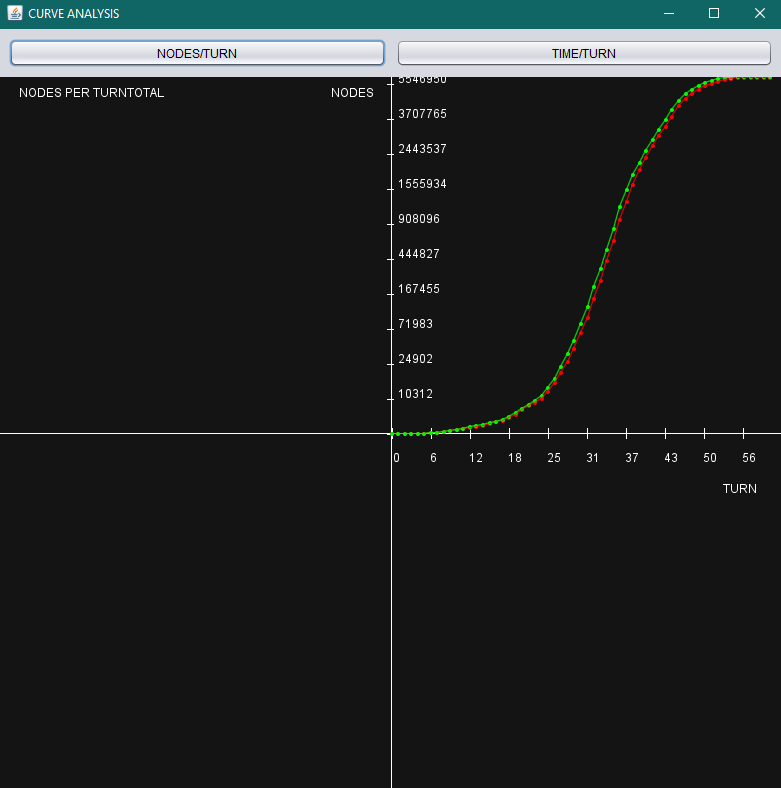
\includegraphics[width=0.60\textwidth]{./NODESPERTURN3}
\end{center}
\end{figure}

\begin{figure}[!ht]
\begin{center}
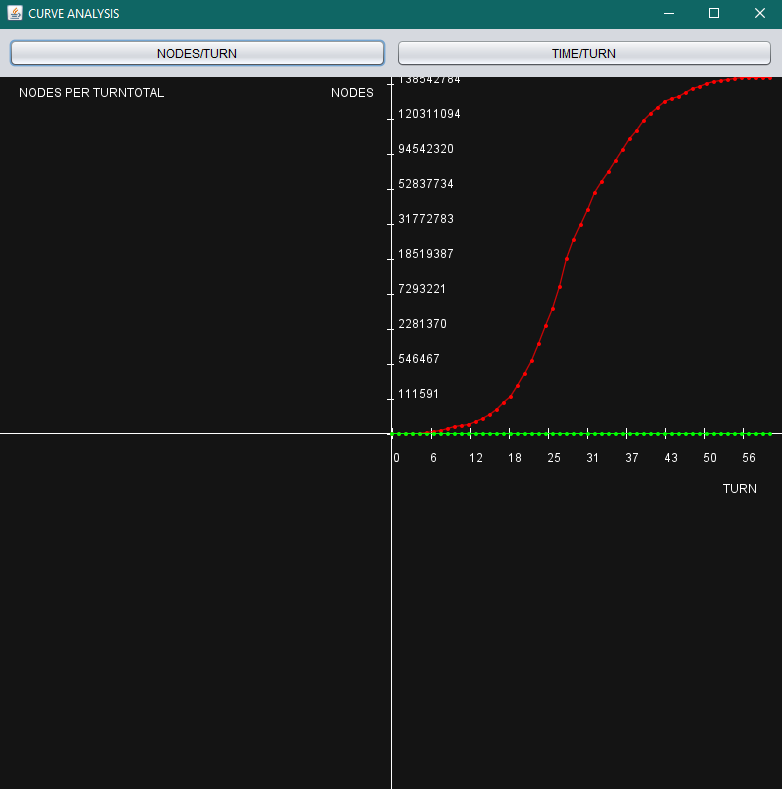
\includegraphics[width=0.60\textwidth]{./NODESPERTURN4}
\end{center}
\end{figure}
\newpage

\textbf{Sur les deuxièmes types de courbes nous voyons le même processus mais sous un autre angle.}

\begin{figure}[!ht]
\begin{center}
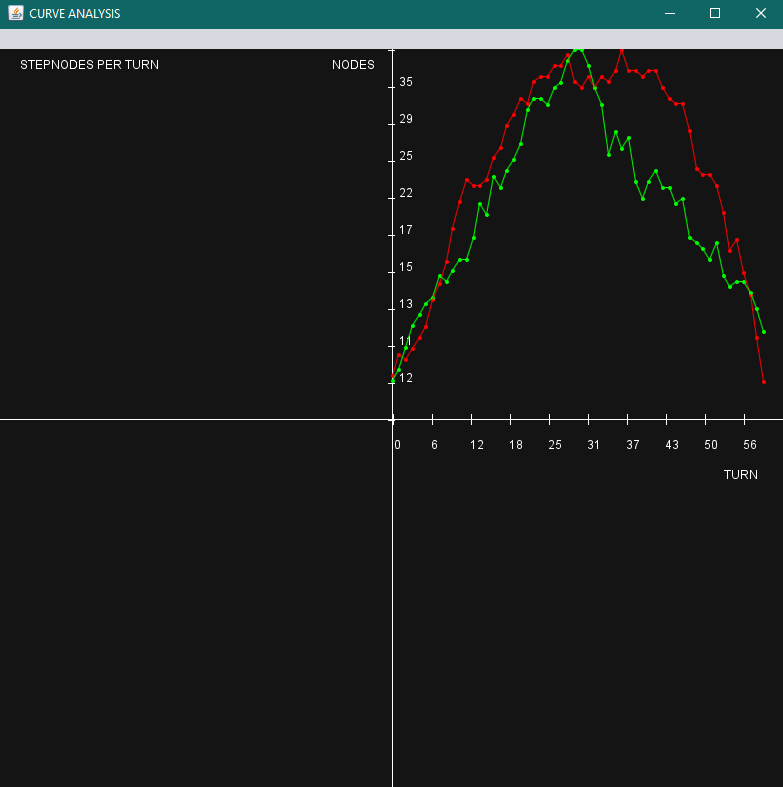
\includegraphics[width=0.60\textwidth]{./STEPNODESPERTURN0}
\end{center}
\end{figure}

\begin{figure}[!ht]
\begin{center}
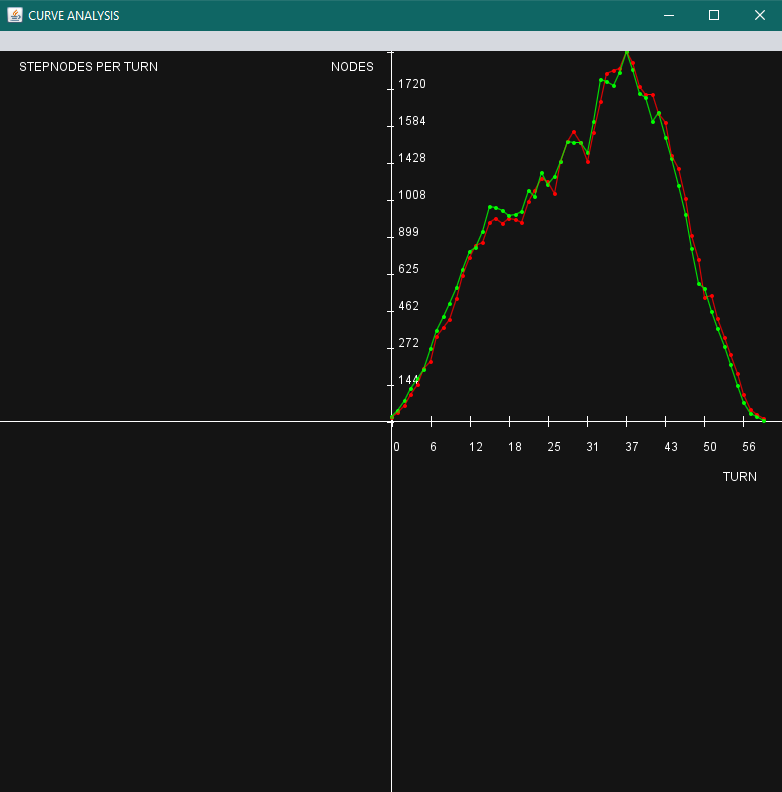
\includegraphics[width=0.60\textwidth]{./STEPNODESPERTURN1}
\end{center}
\end{figure}
\newpage

\begin{figure}[!ht]
\begin{center}
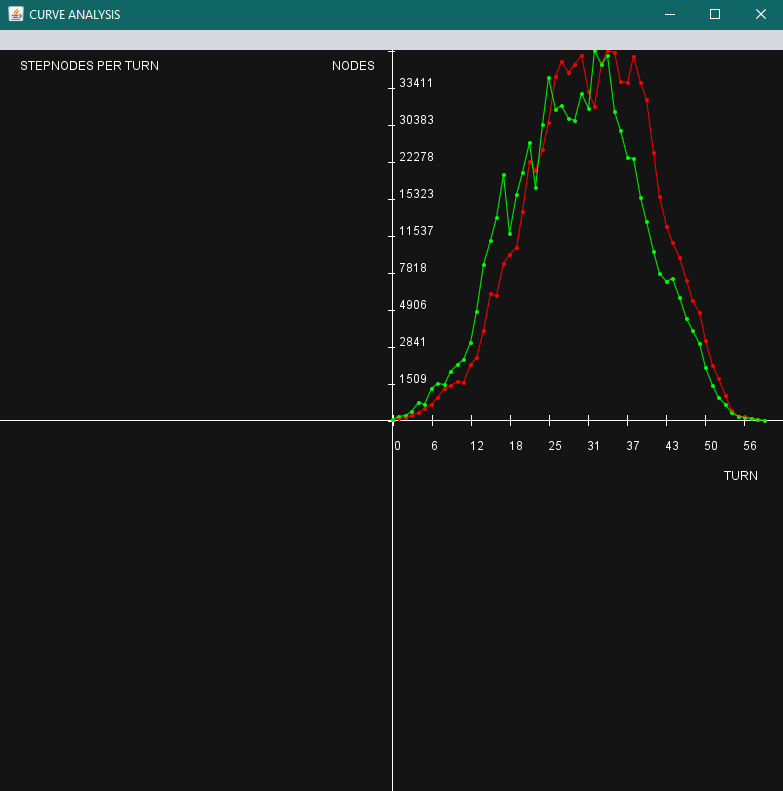
\includegraphics[width=0.60\textwidth]{./STEPNODESPERTURN2}
\end{center}
\end{figure}

\begin{figure}[!ht]
\begin{center}
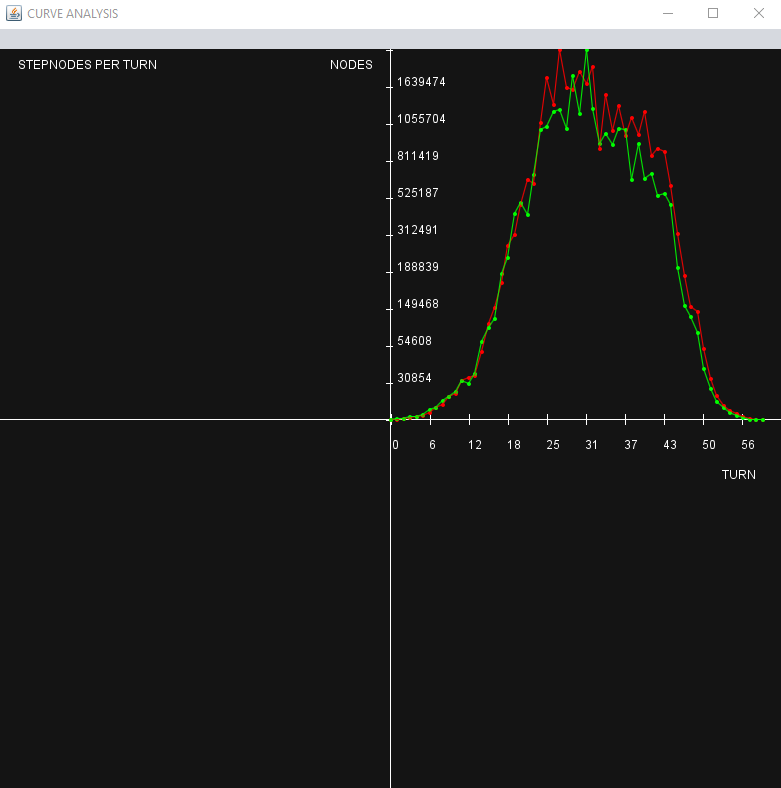
\includegraphics[width=0.60\textwidth]{./STEPNODESPERTURN3}
\end{center}
\end{figure}

\newpage

\begin{figure}[!ht]
\begin{center}
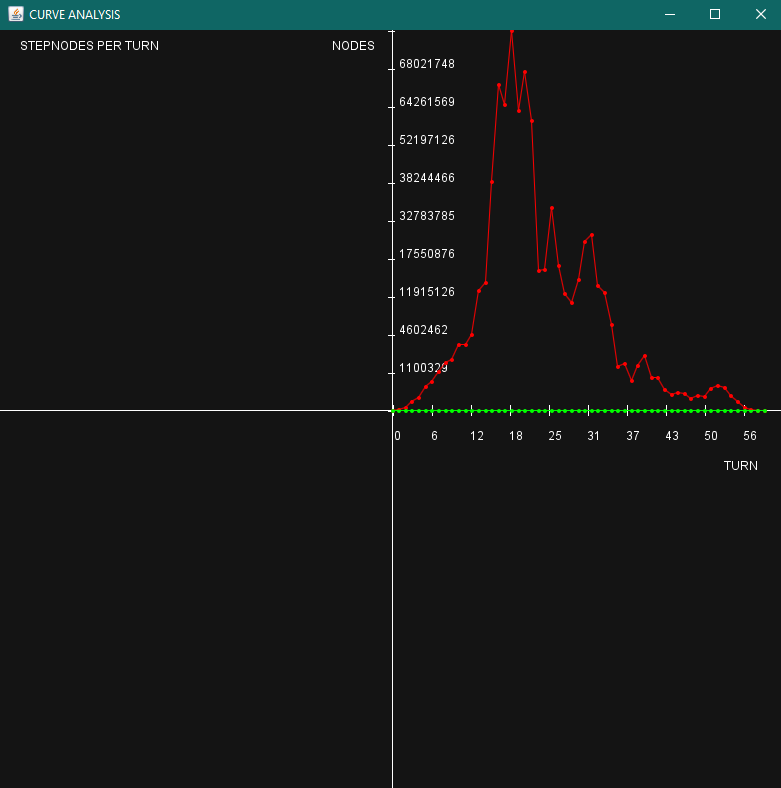
\includegraphics[width=0.65\textwidth]{./STEPNODESPERTURN4}
\end{center}
\end{figure}

Si nous avions réussit à implémenter alphabeta nous aurions tracé les courbes avec deux joueurs de même
profondeur minmax, mais l'un avec alphabeta activé et l'autre sans.
Nous aurions donc observé que la courbe du joueur avec alphabeta activé aurait été en dessous de l'autre
joueur.

\newpage

\subsection{Par profondeur}

Pour comprendre à quel point le nombre de nœuds croît suivant la profondeur donnée à l'algorithme,
nous avons tracé les courbes des nombres de nœuds totaux par rapport à la profondeur donnée à
MinMax. \\[0.75 cm]

 
\centering \textbf{Profondeur 0}
\begin{figure}[!ht]
\begin{center}
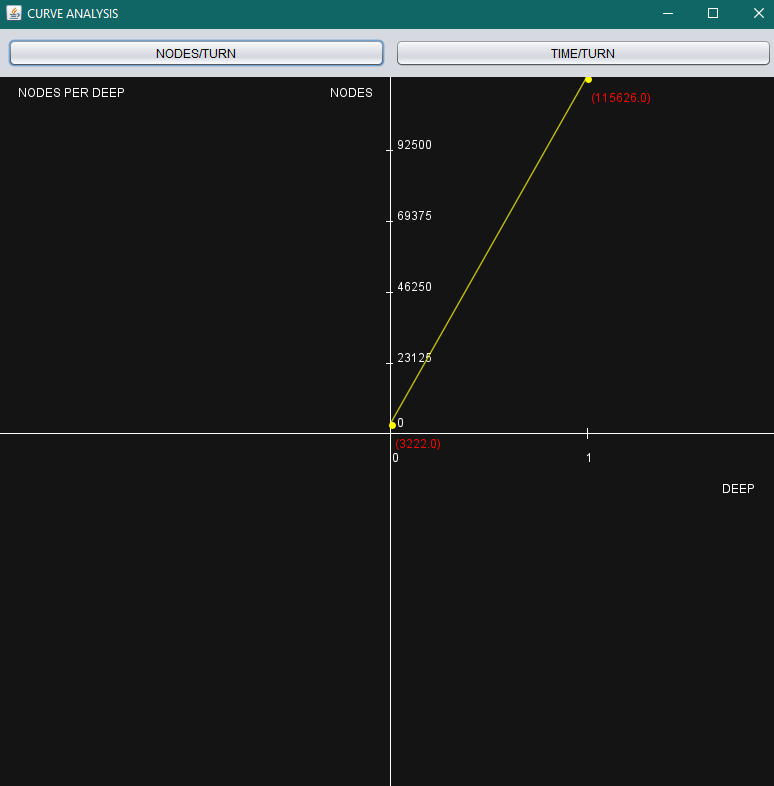
\includegraphics[width=0.60\textwidth]{./NODESPERDEEP1}
\end{center}
\end{figure}

\centering \textbf{Profondeur 1}
\begin{figure}[!ht]
\begin{center}
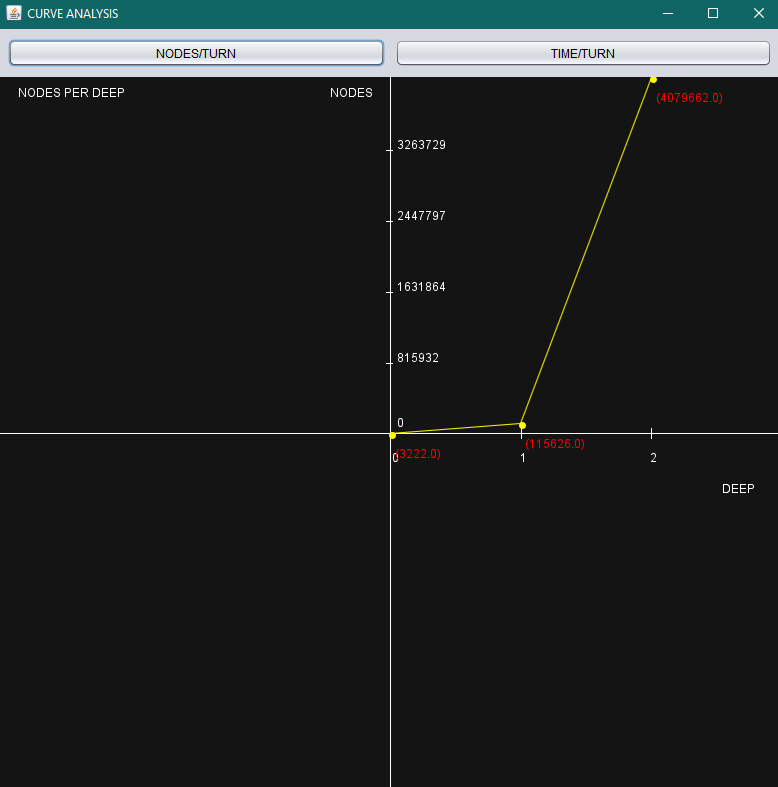
\includegraphics[width=0.60\textwidth]{./NODESPERDEEP2}
\end{center}
\end{figure}
\newpage

\centering \textbf{Profondeur 3}
\begin{figure}[!ht]
\begin{center}
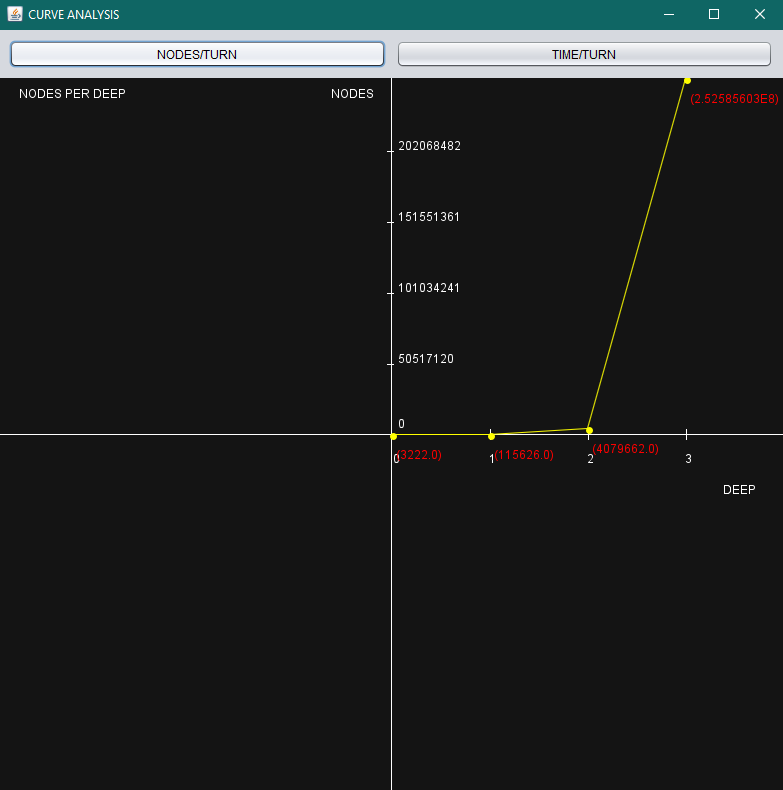
\includegraphics[width=0.60\textwidth]{./NODESPERDEEP3}
\end{center}
\end{figure}

Nous observons ici des courbes exponentiels, ceci étant logique vu que le nombre de nœuds explorés
est égale à: CoupsValidesAvecTour\up{profondeur} 
\newpage


\section{Taux de victoire par rapport a la profondeur et au nombre de coups d'avance}
Les captures suivantes sont des analyses de plusieurs parties suivant la profondeur et le nombre
de coups d'avance.
Ces parties ont toutes été jouées sur des grille de taille (11,11), CD veut dire "Coups d'avances" dans
ces tableaux.

\centering \textbf{MinMax 1 vs MinMax 0}
\begin{figure}[!ht]
\begin{center}
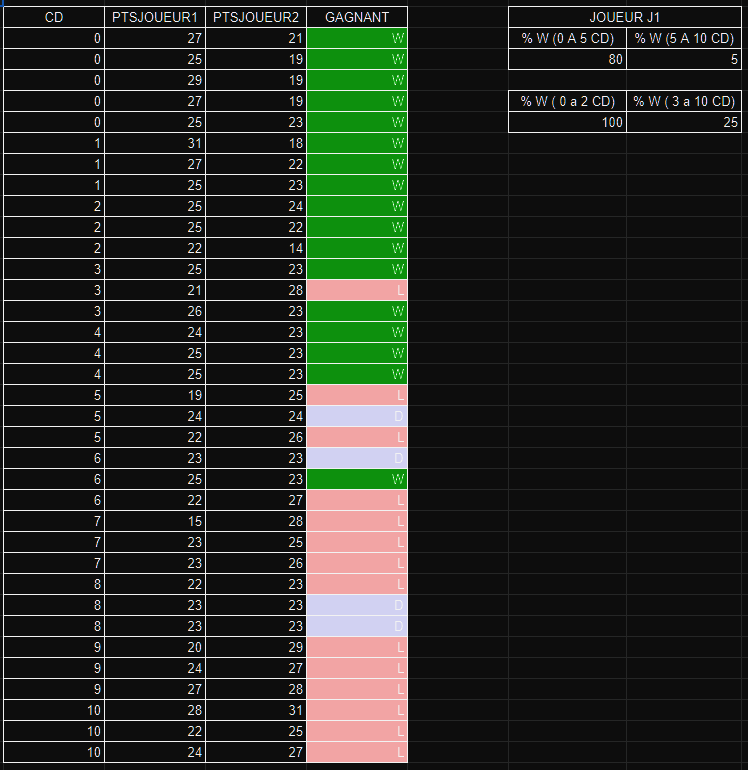
\includegraphics[width=0.70\textwidth]{./TABLEURDEEP1}
\end{center}
\end{figure}
\newpage


\centering \textbf{MinMax 2 vs MinMax 0}
\begin{figure}[!ht]
\begin{center}
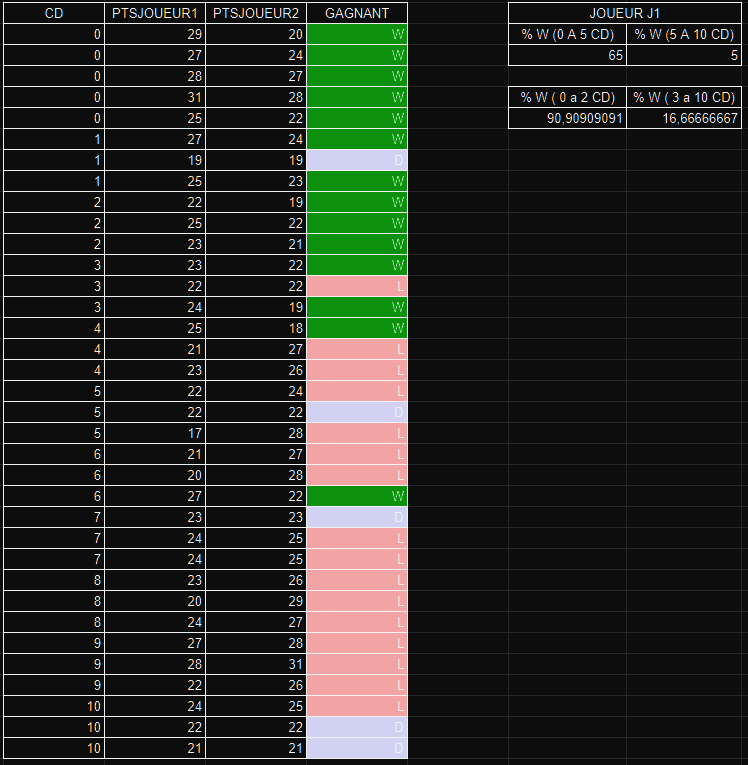
\includegraphics[width=0.70\textwidth]{./TABLEURDEEP2}
\end{center}
\end{figure}
\newpage

\centering \textbf{MinMax 3 vs MinMax 0}
\begin{figure}[!ht]
\begin{center}
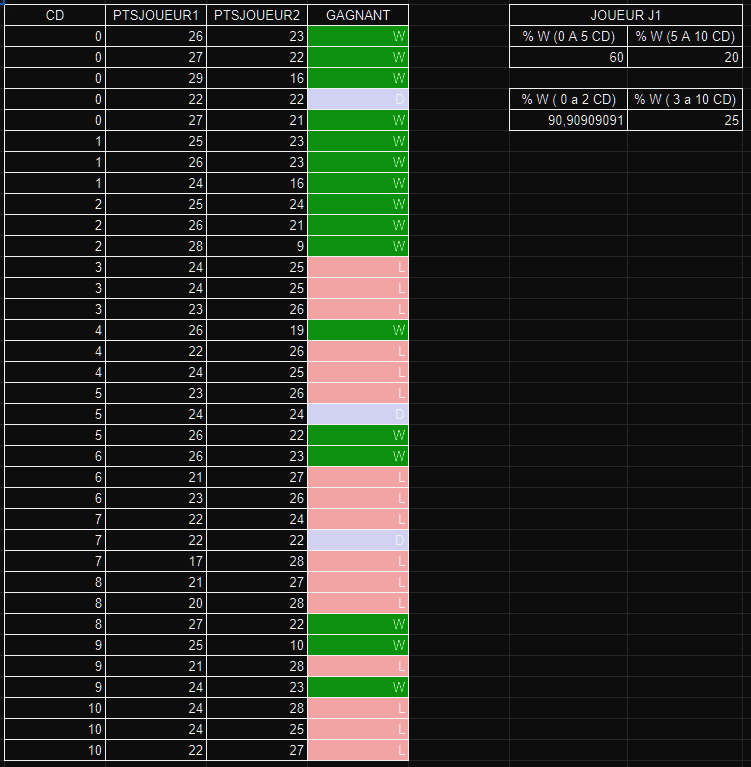
\includegraphics[width=0.70\textwidth]{./TABLEURDEEP3} 
\end{center}
\end{figure}


D'après ces tableaux on peut voir que lorsque l'on donne moins de 3 coups d'avances au joueur MinMax0
MinMax1 gagne toujours. Alors que pour plus de 3 coups d'avances, MinMax0 commencent à battre MinMax1.
Cela fonctionne pareil pour MinMax2 et MinMax3.
Avec des analyses plus poussées, nous aurions pu faire beaucoup d'autre tableur comme ceux-ci, mais 
en changeant la taille de la grille. Grâce a cela nous aurions peu être pu mettre en évidence 
une corrélation entre la taille de la grille et le nombre de coups d'avance.

\newpage
\section{analyse de temps}

Nous avons récupéré des données sur les temps maximums de décisions de MinMax suivant la profondeur
donnée.
Premièrement nous avons afficher a chaque fin de partie le temps maximum de MinMax pour choisir un coup,
le temps total de la partie ainsi que des informations sur le nombre de nœuds parcourus.

\begin{figure}[!ht]
\begin{center}
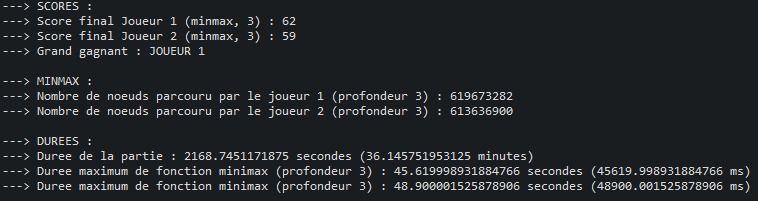
\includegraphics[width=0.70\textwidth]{./EXEMPLEANALYSEFINPARTIE}
\end{center}
\end{figure}

Puis nous avons tracé des courbes après avoir récupéré ces données avec plusieurs profondeurs données :





\begin{figure}[!ht]
\begin{center}
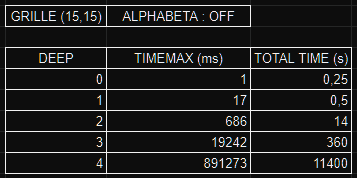
\includegraphics[width=0.70\textwidth]{./TABLEURDONNEESCOURBES} 
\end{center}
\end{figure}

\begin{figure}[!ht]
\begin{center}
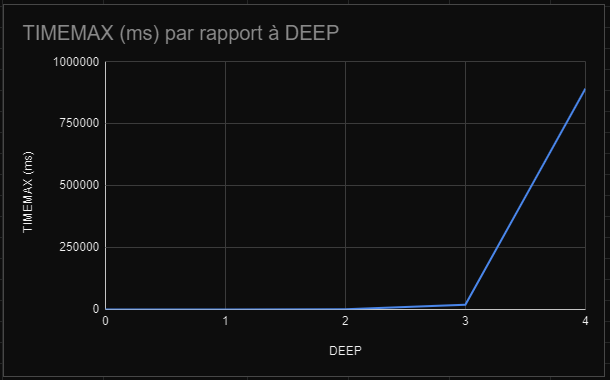
\includegraphics[width=0.70\textwidth]{./TIMEMAXPERDEEP} 
\end{center}
\end{figure}
\newpage

\begin{figure}[!ht]
\begin{center}
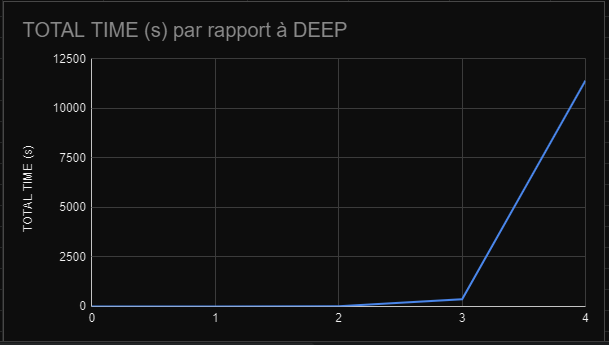
\includegraphics[width=0.70\textwidth]{./TOTALTIMEPERDEEP}
\end{center}
\end{figure}

\textbf{Ces courbes ressemblent fortement aux courbes du 1.1.2, la rapidité du MinMax en temps étant liée au nombre de nœuds parcourus.}



























